\documentclass[pdf, aspectratio=169, 12pt]{beamer}
\usepackage[]{hyperref, graphicx, siunitx, lmodern, tikz, booktabs, physics}
\usepackage[mode=buildnew]{standalone}
\usepackage{pdfpc-commands}
\usepackage{pgfplots}
\pgfplotsset{compat=1.16}

\usetheme{Python}

\graphicspath{ {Images/} }

\sisetup{per-mode=symbol}
\usetikzlibrary{calc, patterns, decorations.markings, decorations.pathmorphing, shapes}


% NOTE THIS LECTURE COMES AFTER THE CH4_1 LECTURE FOR HOMEWORK PURPOSES!


%Preamble
\title{Newton does it all (with help)}
\author{Jed Rembold}
\date{February 19, 2020}

\begin{document}

\begin{frame}{Announcements}
	\begin{itemize}
		\item Homework
			\begin{itemize}
				\item I'm still working on the HW3 grading, sorry. 
				\item Be working on Homework 4!
					\begin{itemize}
						\item Problem 3 should be doable at least up till the animation
						\item Problem 2 doable after today
						\item Pieces of Problem 1 doable after today
					\end{itemize}
			\end{itemize}
		\item No presenter for CS Tea tomorrow, and it is just out in the meeting area between offices
			\begin{itemize}
				\item Still pizza, cookies, and goodies though!
				\item 11:35am
			\end{itemize}
		\item Polling: \url{rembold-class.ddns.net}
	\end{itemize}
\end{frame}

\begin{frame}[fragile]{Review Question}
	\begin{columns}
		\column{0.5\textwidth}
		When the final line of the code to the right is run, what type of variable is \pyi{x}?
		\begin{poll}
			\item \texttt{integer}
			\item \texttt{float}
			\item \texttt{string}
			\item \texttt{NoneType}
		\end{poll}
		\exsol{\texttt{NoneType}}
		
		\column{0.5\textwidth}
		\begin{pythoncode}
			def func(A):
				m = str(A)
				n = m * 10
				print(n)

			y = 5.0
			x = func(y)
			print(type(x))
		\end{pythoncode}
	\end{columns}
	
\end{frame}

\begin{frame}{Convergence}
	\begin{center}
		\begin{tikzpicture}
			\begin{axis}[
				width = \textwidth,
				height = 7cm,
				xlabel = Iterations,
				ylabel = Distance from Target,
				legend style = {fill=BG, draw = Purple},
				legend pos = south east,
				grid = major,
				grid style = {dotted}
				]
				\addplot[Blue,mark=*] table[x=Iter, y=Exh, col sep=comma] {Data/Convergence.csv};
				\addplot[Orange,mark=*,sharp plot] table[x=Iter, y=Bis, col sep=comma] {Data/Convergence.csv};
				\legend{Exhaustive Enumeration, Bisection Search}
			\end{axis}
		\end{tikzpicture}
	\end{center}
\end{frame}

\begin{frame}{Newton-Raphson}
	\begin{itemize}
		\item Alternative method to find roots of polynomials
			\[f(x) = 4x^3 + 2x + 10\]
		\item Requires an initial guess to work, but \emph{does not require explicit bounds}!
		\item Revolves around the idea that, if \pyi{g} is a guess for the root of $f(x)$, then
			\[g - \frac{f(g)}{f^\prime(g)}\]
			is an even better guess.
	\end{itemize}
\end{frame}

\begin{frame}{Mathematical Understanding}
	\begin{itemize}
		\item Need to find the derivative (probably analytically for the time being.
			\begin{itemize}
				\item For polynomials of form $f(x) = Ax^n$,
					\[f^\prime(x) = Anx^{n-1}\]
				\item Derivatives of sums add. If $f(x) = g(x) + h(x)$:
					\[f^\prime(x) = g^\prime(x) + h^\prime(x)\]
				\item Can always use an online calculator if your derivatives are shakey
			\end{itemize}
	\end{itemize}
\end{frame}

\begin{frame}[fragile]{Implementation Example}
	\begin{example}
		Find the point where $8x^2 = 3$ with epsilon = 0.01.
	\end{example}
	\pause

	\begin{pythoncode}
		guess = 1
		epsilon = 0.01
		while abs(8*guess**2 - 3) > epsilon:
			val = 8*guess**2 - 3
			deriv = 16*guess
			guess = guess - val/deriv
		print(guess)
	\end{pythoncode}
\end{frame}

\begin{frame}[fragile]{Return of the Cube Root of 27}
	\begin{example}
		Let's return again to computing the cube root of 27, but this time using the Newton-Raphson algorithm. We'll look for a solution that works for an epsilon of 0.01.
	\end{example}
\end{frame}

\begin{frame}{Comparison}
	\begin{center}
		\begin{tikzpicture}
			\begin{axis}[
				ymin = -50,
				ymax = 50,
				width = \textwidth,
				height = 7cm,
				xlabel = Iterations,
				ylabel = Distance from Target,
				legend style = {fill=BG, draw = Purple},
				legend pos = north east,
				grid = major,
				grid style = {dotted}
				]
				\addplot[Orange, mark=*] table [x=Iter, y=Bis, col sep=comma] {Data/Convergence2.csv};
				\addplot[Blue, mark=*] table [x=Iter, y=Newt, col sep=comma] {Data/Convergence2.csv};
				\legend{Bisection Search, Newton-Raphson}
			\end{axis}
		\end{tikzpicture}
	\end{center}
\end{frame}

\begin{frame}{Be Careful}
	\begin{itemize}
		\item Realize that any numeric method we have looked at will only get you a \alert{single} solution!
		\item How do you work with equations that might have multiple possibilities?
			\begin{itemize}
				\item You have to separate them out with separate ranges or guesses
				\item Frequently might mean it would be useful to look at a quick plot of a function to understand near where certain roots exist
					\begin{itemize}
						\item We'll learn to plot in Python more later in the semester, but for now you can always use something like Desmos or WolframAlpha
					\end{itemize}
			\end{itemize}
		\item Remember your expressions should be equal to 0
		\item Be careful of points with slope 0, as if you should hit them exactly your algorithm will break.
	\end{itemize}
\end{frame}

\begin{frame}{Multiroot Example}
	\begin{columns}
		\column{0.5\textwidth}
		\begin{example}
			Suppose you want to find when
			\[(x+3)^3 +5x^2 - 15x - 100 = 100\]
			when epsilon = 0.1. Find all real solutions.
		\end{example}
		\column{0.5\textwidth}
		\begin{center}
			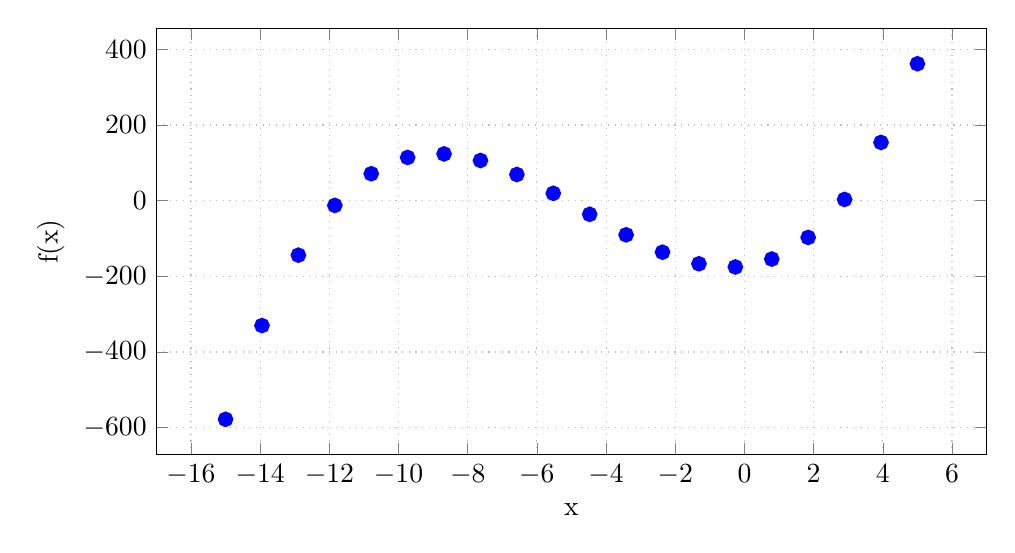
\begin{tikzpicture}
				\begin{axis}[
					width = \textwidth,
					height = 7cm,
					xlabel = x,
					ylabel = f(x),
					legend style = {fill=BG, draw = Purple},
					legend pos = north east,
					grid = major,
					grid style = {dotted}
					]
					\addplot[domain=-15:5, samples=20,Blue, ultra thick, only marks] 
						{(x+3)^3 + 5*x^2 -15*x - 200};
				\end{axis}
			\end{tikzpicture}
		\end{center}
	\end{columns}
\end{frame}

\section{Back to Chapter 4!}

\begin{frame}[fragile]{The Word is Key}
	\vspace{5mm}
	\begin{itemize}[<+->]
		\item So far we have looked at a positional way to assign arguments to formal parameters
			\begin{itemize}
				\item The first argument to the first parameter, the second to the second, etc
					\begin{center}
						\begin{pythoncode}
							def func(first, second, third):
								print(first, second, third)

							func(1,2,3)
							func(2,6,4)
						\end{pythoncode}
					\end{center}
			\end{itemize}
		\item Can also write explicitly with keyword arguments!
			\begin{itemize}
				\item If you do so, the position no longer matters
					\begin{center}
						\begin{pythoncode}
							func(third=4, first=2, second=6)
						\end{pythoncode}
					\end{center}
			\end{itemize}
		\item \textcolor{Red}{All keyword arguments must come after any positional arguments!}
	\end{itemize}
\end{frame}

\begin{frame}[fragile]{Default Slide Title}
	\begin{itemize}[<+->]
		\item Can also specify default values for a formal parameter
			\begin{pythoncode}
				def func(name='Jed', age=34)
					print('My name is', name, 'and I am', age)
			\end{pythoncode}
		\item You then don't need to always provide that actual parameter
		\item If setting any parameters out of order though, you \alert{must} indicate them through keywords.
			\begin{pythoncode}
				func()
				func('Bob',25)
				func('Larry')
				func(age=68)
			\end{pythoncode}
	\end{itemize}
\end{frame}

\end{document}

